\documentclass[10pt,twocolumn,twoside]{phdsymp-en}
\usepackage[utf8]{inputenc}
\usepackage[english]{babel}
\usepackage{times}
\usepackage{enumitem}
\usepackage[hang,flushmargin]{footmisc} 
\usepackage{microtype}
\usepackage[dvipsnames]{xcolor}
\usepackage{amsmath}
\usepackage{amssymb}
\usepackage{tikz}
\renewcommand{\baselinestretch}{1.1}
\def\BibTeX{{\rm B\kern-.05em{\sc i\kern-.025em b}\kern-.08em
		T\kern-.1667em\lower.7ex\hbox{E}\kern-.125emX}}
\renewcommand{\familydefault}{\sfdefault}
\usepackage{caption}
\usepackage[list=true]{subcaption}
\usepackage{fontawesome5}
\usepackage[detect-weight=true, binary-units=true, range-phrase=-]{siunitx}
\usepackage{tabularx}
\usepackage{tikz}
\usepackage{tikzscale}
\usepackage[final]{hyperref}
\usepackage{cleveref}

% Table columns.
\newcolumntype{C}{>{\centering\arraybackslash}X}

% Subcaptions.
\captionsetup{compatibility=false}

% Tikz libraries.
\usetikzlibrary{arrows,arrows.meta,automata,calc,shapes.geometric,positioning}

% Colours.
\definecolor{black}{RGB}{0, 0, 0}
\definecolor{bisque}{HTML}{FFE4C4}
\definecolor{code-background}{HTML}{EEEEEE}
\definecolor{code-delim}{RGB}{20,105,176}
\definecolor{darkgray}{rgb}{.4,.4,.4}
\definecolor{groovyblue}{HTML}{0000A0}
\definecolor{groovygreen}{HTML}{008000}
\colorlet{code-punct}{red!60!black}
\definecolor{ugent-blue}{RGB}{30, 100, 200}

% Meta-information.
\hypersetup{
	pdfauthor = {Pieter De Clercq},
	pdftitle = {Optimising Continuous Integration using Test Case Prioritisation},
	pdfsubject = {Master's dissertation submitted in order to obtain the academic degree of Master of Science in Computer Science, june 2020},
	linkcolor = black,
	citecolor = ugent-blue,
	urlcolor = ugent-blue,
	colorlinks = true,
}

% Terms.
\newcommand{\travisci}{Travis CI}
\newcommand{\velocity}{VeloCIty}

\begin{document}
	\title{Optimising Continuous Integration\\ using Test Case Prioritisation}
	\author{Pieter De Clercq}
	\supervisor{Prof. dr. B. Volckaert, Prof. dr. ir. F. De Turck, J. Vaneessen, D. Kerkhove}
	\maketitle
	
	\begin{abstract}
	Ever since the introduction of traditional software development models in the previous century, the complexity and magnitude of today's software have vastly increased. This evolution has led to the adoption of Agile software development approaches, which pose the need for frequent integration and automated testing. Eventually, this increase in size will also negatively affect the size of the testing suites, resulting in severe scalability issues. This thesis proposes a framework and a novel algorithm for test suite optimisation by prioritising test cases which are likely to fail. The performance has been evaluated on two existing applications, and the results are auspicious.
	\end{abstract}

	\begin{keywords}
		Continuous Integration, test suite, performance, optimisation, prioritisation
	\end{keywords}

	% !TeX root = thesis.tex

\chapter{Introduction}
\label{ch:introduction}
Given the complexity and rapid pace at which software is being built today, it is inevitable that sooner or later, bugs will emerge. These bugs can either be introduced by a malfunctioning new feature, or by breaking existing functionality (\emph{a regression}). In order to detect bugs in an application before its users do, we require an adequate \emph{testing infrastructure}.\\

\noindent This testing infrastructure consists of multiple \emph{test cases}, collectively referred to as the \emph{test suite} of the application. The quality of a test suite can be assessed in multiple ways. The first and most commonly used method is to measure which fraction of the source code is tested by at least one test case, a ratio which is indicated as the \emph{coverage} of the application. Another possibility is to apply transformations to the source code and validate whether or not this results in a failed test case, a process indicated as \emph{mutation testing}.\\

\noindent Ideally, this testing process should be automated and performed after every change to the source code. This process is generally very time-consuming, and as such has led to the creation of various automation frameworks and tools, collectively called \acrfull{ci}. Common examples of \acrshort{ci} practices are automatically running the test suite and estimating the code coverage after every pushed change to the \acrfull{vcs}.\\

\noindent However, applying these practices and maintaining a qualitative test comes at a cost. Every addition or modification to the source code must be followed by at least one test case to validate its correctness. As a result of the speed at which the source code tends to grow, the test suite suffers from severe scalability issues. While it is desirable and ideally required to execute every single test case in the test suite, there are examples known to literature where this is not possible since this incurs an increasing delay in the development process, which in turn results in economic loss.\\

\noindent We can take three approaches to resolve this issue and reduce the time waiting for the test results: \acrfull{tsm}, \acrfull{tcs} and \acrfull{tcp}. The main subject of this thesis will be to implement a framework for \acrshort{tcp}.

\noindent The structure of this thesis is as follows. The next chapter will introduce essential concepts used in modern software engineering. \Cref{ch:related-work} will elaborate more on the three mentioned approaches and present accompanying algorithms. The implementation details of the new framework will be discussed in \Cref{ch:velocity}. Afterwards, \Cref{ch:evaluation} will evaluate the performance of this framework and provide insights into the characteristics of a typical test suite. More specifically, this chapter will investigate the probability of (repeated) test failure and the average duration of a test run. Finally, \Cref{ch:conclusion} will present additional ideas and improvements to the framework.
	\section{Techniques}
\noindent This thesis presents three techniques to solve this problem.

\begin{figure*}[t]
	\centering
	\subcaptionbox{Test Suite Minimisation}{\includegraphics[width=0.32\textwidth]{assets/tsm.tikz}}
	\hfill
	\subcaptionbox{Test Case Selection}{\includegraphics[width=0.32\textwidth]{assets/tcs.tikz}}
	\hfill
	\subcaptionbox{Test Case Prioritisation}{\includegraphics[width=0.32\textwidth]{assets/tcp.tikz}}
	\caption{Illustration of the techniques.}
\end{figure*}

\subsection{Test Suite Minimisation (TSM)}
\noindent The first technique is called Test Suite Minimisation (TSM) \cite{10.1002/stv.430}. TSM will attempt to reduce the size of the test suite by permanently removing redundant test cases according to the following definition:\\

\noindent\fbox{\begin{minipage}{\columnwidth}
\textbf{Given:}
\begin{itemize}
	\item $T = \{t_1, \dots, t_n\}$ a test suite consisting of test cases $t_j$.
	\item $R = \{r_1, \dots, r_m\}$ a set of requirements that must be satisfied in order to provide the desired ``adequate'' testing of the program.
	\item $\{T_1, \dots, T_m\}$ subsets of test cases in $T$, one associated with each of the requirements $r_i$, such that any one of the test cases $t_j \in T_i$ can be used to satisfy requirement $r_i$.
\end{itemize}
\mbox{}\\
TSM is then defined as the task of finding a subset $T'$ of test cases $t_j \in T$ that satisfies every requirement $r_i$.
\end{minipage}}

\subsection{Test Case Selection (TCS)}
\noindent Instead of permanently removing redundant test cases, it is also possible to analyse the code changes and deduce which test cases should be executed and which might ones be omitted altogether. This technique is referred to as Test Case Selection (TCS) \cite{10.1002/stv.430}.\\

\noindent\fbox{\begin{minipage}{\columnwidth}
\textbf{Given:}
\begin{itemize}
	\item $T$ the test suite.
	\item $P$ the previous version of the codebase.
	\item $P'$ the current (modified) version of the codebase.
\end{itemize}
\mbox{}\\
TCS aims to find a subset $T' \subseteq T$ that is used to test $P'$. 
\end{minipage}}

\subsection{Test Case Prioritisation (TCP)}
\noindent While TSM and TCS execute only the relevant test cases, sometimes it might be required that every test case is successfully executed. Consider, for example, critical software for medical purposes. In this case, it is still possible to optimise the test suite by executing all test cases in a specific order. Test Case Prioritisation (TCP) \cite{10.1002/stv.430} constructs an ordered sequence that aims to fulfil a predetermined objective as fast as possible. This thesis primarily uses the detection of the first failed test case as the objective.\\

\noindent\fbox{\begin{minipage}{\columnwidth}
\textbf{Given:}
\begin{itemize}
	\item $T$ the test suite.
	\item $PT$ the set of permutations of $T$.
	\item $f: PT \mapsto \mathbb{R}$ a function from a subset to a real number, this function is used to compare sequences of test cases to find the optimal permutation.
\end{itemize}
\mbox{}\\
TCP finds a permutation $T' \in PT$ such that $\forall T'' \in PT : f(T') \ge f(T'') \Rightarrow (T'' \ne T')$. 
\end{minipage}}
	\section{Algorithms}
\noindent This thesis prefers to use TCP since this technique does not incur the risk of false-negative failing test cases. In order to determine the optimal order of execution, this thesis presents three existing algorithms.\\

\noindent The input data for these algorithms is threefold:\\

\begin{itemize}
\item \textbf{Affected test cases:} By combining previous coverage results and the list of changes that the developer has made to the code, the framework can estimate which test cases are likely affected by those changes and assign a higher priority.

\item \textbf{Historical data:} Next, historical failure data can be used. Suppose that a test case has failed in its previous execution, then there exists a chance that it will subsequently fail in the current run.

\item \textbf{Execution timings:} Finally, if two test cases are considered equally likely to fail, the average duration of the test case can be used as a tie-breaker. Since the objective of TCP is to optimise the test suite, the test case with the lowest duration should be preferred.
\end{itemize}

\subsection{Greedy algorithm}
\noindent The first algorithm is a greedy heuristic that was initially designed as an algorithm for the set-covering problem \cite{evaluationoftestsuiteminimization}. This heuristic starts with an empty set of test cases and the set of all code lines $C$. Next, the algorithm iteratively selects the test case that contributes the most code lines that are not yet covered, updating $C$ after every selected test case. The algorithm halts when either all test cases are selected or $C$ is empty. In order to modify this algorithm to make it applicable to TCP, the selection order must be preserved and used as the prioritised sequence.

\subsection{HGS algorithm}
\noindent The second algorithm was created by Harrold, Gupta and Soffa \cite{hgs}. As opposed to the greedy heuristic, this algorithm uses a different perspective. First, the algorithm sorts the code lines increasingly based on the number of test cases that cover them. The motivation for this sorting operation is that some test cases must inevitably be executed, as they are the only test cases that cover a given set of lines. However, these test cases can also cover other lines and therefore make other test cases redundant. The algorithm iterates over the code lines in this order and selects one corresponding test case in each iteration. Afterwards, the order is updated to remove source code lines which are now covered by the selected test case. This process is repeated until there are no lines left to cover.

\clearpage

\subsection{ROCKET algorithm}
\noindent Finally, this thesis considers the ROCKET algorithm \cite{6676952}. This algorithm prioritises test cases by assigning a score to every test case, which is calculated using historical failure data. Afterwards, the algorithm computes the cumulative score $CS_t$ of every test case $t$ and defines the following objective function $g$, in which $E_t$ represents the execution time of the test case:
$$g = (maximise(CS_t), minimise(E_t))$$

\noindent Finally, the algorithm optimises this function to determine the ideal order of execution $S$, as follows:
$$(\forall i \in 1 \dots n)(g(S_i) \ge g(S_{i+1})$$
	\section{Framework}
\noindent This thesis proposes a language-agnostic framework that enables Test Case Prioritisation on existing software projects. The architecture consists of three main components, a meta predictor, and a novel prioritisation algorithm.

\subsection{Agent}
\noindent The first component is the agent. This component hooks into the testing framework of the application to execute the test cases in the required order. The agent obtains the optimal execution sequence by communicating with the next component, which is the controller.

\subsection{Controller}
\noindent The controller is a daemon which performs two tasks. First, the controller listens for requests from agents and acts as a relay to the predictor daemon. Additionally, the controller receives feedback from the agent after every executed test run. This information is used to update the meta predictor, which will be described later.

\subsection{Predictor}
\noindent The final main component of the architecture is the predictor daemon. This component is responsible for interpreting the code changes and determining the optimal order of execution using ten built-in prediction algorithms. These algorithms are variations of the three discussed algorithms, as well as the Alpha algorithm.

\subsection{Meta predictor}
\noindent Since the predictor daemon contains multiple prediction algorithms, a small extra component is required to decide which sequence should be preferred as the final execution order. The meta predictor is a table which assigns a score to every prediction algorithm. The final execution order is the one that has been predicted by the prediction algorithm with the highest score. The controller evaluates the performance of every algorithm in the feedback phase, as mentioned before, and updates the scores accordingly.

\subsection{Alpha algorithm}
\noindent In addition to the Greedy, HGS and ROCKET algorithms, the framework features a custom prioritisation algorithm as well. This algorithm starts by inspecting the changed code lines to obtain the affected test cases $ATS$. Among $ATS$, the algorithm selects every test case that has failed at least once in its previous three executions and sorts those by increasing execution time. Next, the algorithm selects the remaining test cases from $ATS$ and sorts those equivalently. After these two steps, the algorithm proceeds like the greedy algorithm until it has processed every test case.
	% !TeX root = ../thesis.tex

\section{Results}

\subsection{RQ1: Probability of failure}\label{ssec:results-rq1}
\autoref{fig:rq1-failure-probability} contains two pie charts that illustrate the amount of failed and successful test runs. The left chart contains the results of the dataset provided by Durieux et al \cite{travisanalysis}. This dataset contains $\SI{4558279}{}$ failed test runs versus $\SI{24323724}{}$ successful runs, which corresponds to a failure probability of $\SI{18.74}{\percent}$. The other pie chart visualises data from the TravisTorrent project. According to this dataset, the run has failed prior to starting the test suite in $\SI{42.89}{\percent}$ of the executions. For the remaining part of the runs, $\SI{225766}{}$ out of $\SI{2114920}{}$ executions contained at least one failed test case, corresponding to a failure percentage of $\SI{10.67}{\percent}$.

\begin{figure}[htbp!]
	\centering
	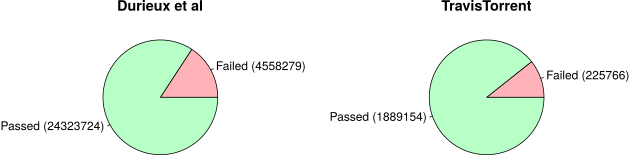
\includegraphics[width=\textwidth]{assets/charts/rq1-failure-probability.pdf}
	\caption{Probability of test run failure}
	\label{fig:rq1-failure-probability}
\end{figure}

\subsection{RQ2: Probability of consecutive failure}
In order to find consecutive failures, only the TravisTorrent project can be used as every entry in this dataset contains the identifier of the previous build which is required to link consecutive builds. The dataset contains $\SI{211040}{}$ test runs of which the test suite of the preceding test run was both executed and contained at least one failed test case. As illustrated in \autoref{fig:rq2-consecutive-failure}, $\SI{109224}{}$ of these test runs failed as well, versus $\SI{101816}{}$ test runs ($\SI{51.76}{\percent}$) that did succeed.

\begin{figure}[htbp!]
	\centering
	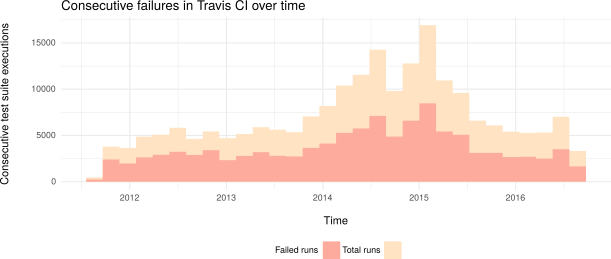
\includegraphics[width=\textwidth]{assets/charts/rq2-consecutive-failure.pdf}
	\caption{Consecutive test run failures on \travisci{}}
	\label{fig:rq2-consecutive-failure}
\end{figure}

\subsection{RQ3: Average test run duration}

maak boxplot van 5.3

- tests lager dan 10 seconden werden genegeerd aangezien dit een failure in de setup betekent.
- de zeer lange tests maken gebruik van mutation testing
- gegroepeerd per hoeveelheid en genormaliseerd op de y-as


\subsection{RQ4: Applying \tcp{} to Dodona}

voor 5.4:

- duration per run
- failed test cases per run
- time (ms) until first failed test case
- time (ms) until first prioritised failed test case
	% !TeX root = thesis.tex

\chapter{Conclusion}
\label{ch:conclusion}

The main purpose of this thesis has been to investigate different approaches towards optimising the test suite of a common software project. The concepts of \tsm{}, \tcs{} and \tcp{} have been introduced and accompanying algorithms have been presented. A novel client-server oriented framework for the latter approach has been proposed, as well as a new prioritisation algorithm. Finally, \velocity{} has been applied to the UGent Dodona project, proving its ability to predict test case failure and therefore reduce the execution time of the test suite.\\

\noindent A second purpose of this thesis was to gain useful insights into the behaviour of a typical test suite. These insights have been formulated as three additional research questions, to which answers have been provided in the previous chapter.

\section{Future work}
The proposed \velocity{} implementation in this thesis is currently able to prioritise a Gradle Java project using 10 available predictors and a meta predictor. While this is certainly functional, it is far from complete and multiple improvements can be added.

\subsection{Java Agent}
The existing Java Agent can be extended in multiple ways. The most prominent addition would be to allow test cases to be executed in parallel. At the moment of writing, this is not possible yet. In order to facilitate parallel testing, one must first decide how to schedule the prioritised test cases across multiple threads, since the execution time of a test case varies strongly. One possibility to perform this scheduling is to use the average execution time per test case, which is obtained from prior runs. Alternatively, this can be performed at runtime by using any existing inter-thread communication paradigm such as message passing. On the implementation side of parallelisation, the current \texttt{TestProcessor} should be adapted to inherit from the \texttt{MaxNParallelTestClassProcessor}. A thread pool should ideally be used to reduce the overhead of restarting a new thread for every test case.

\subsection{Predictions}
Further research and improvements to the predictors can be made on four different aspects.\\

\noindent The first enhancement is that currently the predictor does not discriminate between a unit test or an integration test. 
Recall that the scope of a unit test is limited to a small fraction of the application and that its execution time is ideally rather low. An integration test however usually takes longer to execute and tests multiple components of the application at once. The predictor could make use of this distinction and assume that a failure in a unit test has a high probability of resulting in a failed integration test as well, hence prioritising unit tests over integration tests.\\

\noindent Secondly, the prediction algorithms currently take into account which source code lines have either been modified or removed in order to prioritise affected test cases. Likewise, test cases of which the code has been modified should also be considered as candidates for prioritisation, as the changed test case might contain a bug as well.\\

\noindent A third and unexplored research opportunity is to investigate the joint performance of multiple prediction algorithms combined. This could be integrated with the existing meta predictor. Instead of assigning a score to the entire prediction, multiple predictions could be intermingled using predefined weights.\\

\noindent The final improvement is to take into account branch coverage in addition to the statement coverage which is currently used. This is a rather complex feature as not every coverage framework is capable of reporting accurately which branches have been covered and which ones have not. A suggested implementation would be to instrument the source code and rewrite every condition of every branch as separate \texttt{if}-statements.

\subsection{Meta predictor}
The proposed meta predictor increases the score of every predictor which predicted an above-average ranking and decreases the score of the other predictors. However, a possible problem with this approach is that the nature of the source code might evolve and change as time progresses. Using the current updating strategy it will take several test suite invocations for an alternative predictor to be preferred by the meta predictor. If a saturating counter would be used instead (\autoref{fig:saturating-counter}), this would be resolved much more quickly, allowing a more versatile meta predictor.

\begin{figure}[htbp!]
	\centering
	
\includegraphics[width=\textwidth]{assets/images/saturating-counter.pdf}
	\caption{Saturating counter}
	\label{fig:saturating-counter}
\end{figure}

In addition to implementing a different update strategy, it might be worth to investigate the use of machine learning or linear programming models as a meta predictor, or even as a prediction algorithm.

\subsection{Final enhancements}
Finally, since some of the implemented algorithms are inherently \tsm{} algorithms rather than prioritisation algorithms, the framework might opt to not execute some test cases at all, whereas now the entire test suite is always executed.\\

\noindent Support for other programming languages and frameworks is possible by implementing new agents. The basic implementation is straightforward to restart the test suite after every executed test case, should test case reordering not be supported natively by the test framework.
	
	\bibliographystyle{phdsymp}
	\bibliography{references}
\end{document}